\documentclass[12pt, a4paper]{article}
\usepackage[utf8]{inputenc}
\usepackage{amsmath}
\usepackage{relsize}
\usepackage{array}
\usepackage{xcolor}
\usepackage{courier}
\usepackage{listings}
\lstset{basicstyle=\footnotesize\ttfamily,breaklines=true}
\lstset{framextopmargin=50pt,frame=bottomline}
\usepackage{tikz}
\usetikzlibrary{calc}
\usepackage{graphicx}
\graphicspath{ {./images/} }
\usepackage{multirow}

\title{CEG3155A Assignment 3}
\author{Jake Wang/*}
\date{\today}

\begin{document}
	\maketitle
	
	\section*{Question I}
	\subsection*{Part a}
	$$P_1 = (ABCDEFGH)$$
	Group the state that yield the same value and output together:
	$$P_2 = (ACDE)(BFG)(H)$$
	Consider the next state for $P_2$:
	\[
		P_2^* =
		\left.
		\begin{cases}
			(BBFG)(CFA)(A), & x = 0 \\
			(CEEA)(DHD)(F), & x = 1
		\end{cases}
		\right.
	\]
	In case $x = 0$, for group $(CFA)$ in $P_2^*$, $C$ and $A$ lead to group (ACDE) in $P_2$, whereas $F$ leads to itself. Therefore, $B$ and $G$ need to be grouped from $F$.
	$$P_3 = (ACDE)(BG)(F)(H)$$
	Consider the next state for $P_3$:
	\[
		P_3^* =
		\left.
		\begin{cases}
			(BBFG)(CA)(F)(A), & x = 0 \\
			(CEEA)(DD)(H)(F), & x = 1
		\end{cases}
		\right.
	\]
	In case $x = 0$, for group $(BBFG)$ in $P_3^*$, $B$ and $G$ lead to group (BG) in $P_3$, whereas $F$ leads to itself. Therefore, $A$, $C$ and $E$ need to be grouped from $D$.
	$$P_4 = (ACE)(D)(BG)(F)(H)$$
	Consider the next state for $P_4$:
	\[
		P_4^* =
		\left.
		\begin{cases}
			(BBG)(F)(CA)(F)(A), & x = 0 \\
			(CEA)(F)(DD)(H)(F), & x = 1
		\end{cases}
		\right.
	\]
	There is no need of further partitioning. The reduced state table is as follows:
	\begin{center}
		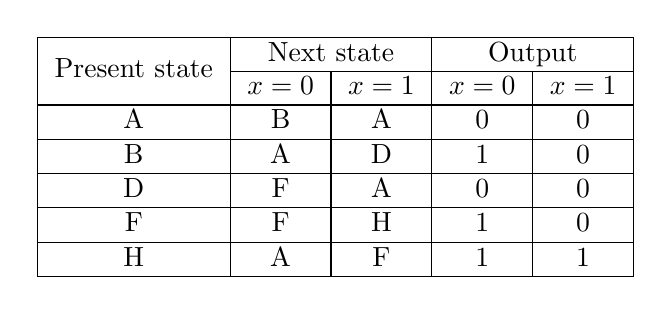
\begin{tikzpicture}
			\node(table)
			{
				\begin{tabular}{| c | c | c | c | c |}
					\hline
					\multirow{2}{*}{Present state} & \multicolumn{2}{c |}{Next state} & \multicolumn{2}{c |}{Output} \\
					\cline{2-5} & $x = 0$ & $x = 1$ & $x = 0$ & $x = 1$\\
					\hline
					A & B & A & 0 & 0 \\
					\hline
					B & A & D & 1 & 0 \\
					\hline
					D & F & A & 0 & 0 \\
					\hline
					F & F & H & 1 & 0 \\
					\hline
					H & A & F & 1 & 1 \\
					\hline
				\end{tabular}
			};
		\end{tikzpicture}
	\end{center}
	
	\subsection*{Part b}
	$$P_1 = (ABCDEFGH)$$
	Group the state that yield the same value and output together:
	$$P_2 = (ACEFH)(BDG)$$
	Consider the next state for $P_2$:
	\[
		P_2^* =
		\left.
		\begin{cases}
			(BAGBF)(DED), & x = 0 \\
			(CFHHE)(ECF), & x = 1
		\end{cases}
		\right.
	\]
	In case $x = 0$, for group $(BAGBF)$ in $P_2^*$, $B$ and $G$ lead to group (BDG) in $P_2$, whereas $A$ and $F$ lead to group (ACEFH). Therefore, $A$, $E$ and $F$ need to be grouped together; $C$ and $H$ need to be grouped together.
	$$P_3 = (AEF)(CH)(BDG)$$
	Consider the next state for $P_3$:
	\[
		P_3^* =
		\left.
		\begin{cases}
			(BGB)(AF)(DED), & x = 0 \\
			(CHH)(FE)(ECF), & x = 1
		\end{cases}
		\right.
	\]
	In case $x = 0$, for group $(DED)$ in $P_3^*$, $D$ leads to group (BDG) in $P_3$, whereas $E$ leads to group (AEF). Therefore, $B$ and $G$ need to be grouped together from $D$.
	$$P_4 = (AEF)(CH)(BG)(D)$$
	Consider the next state for $P_4$:
	\[
		P_4^* =
		\left.
		\begin{cases}
			(BGB)(AF)(DD)(E), & x = 0 \\
			(CHH)(FE)(EF)(C), & x = 1
		\end{cases}
		\right.
	\]
	There is no need of further partitioning. The reduced state table is as follows:
	\begin{center}
		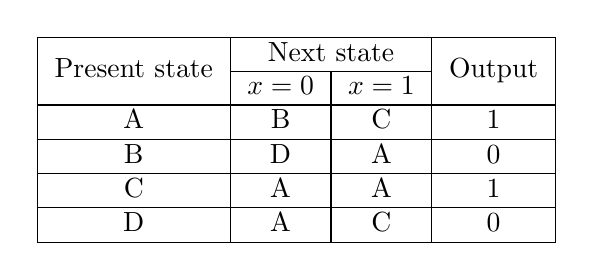
\begin{tikzpicture}
			\node(table)
			{
				\begin{tabular}{| c | c | c | c | c |}
					\hline
					\multirow{2}{*}{Present state} & \multicolumn{2}{c |}{Next state} & \multirow{2}{*}{Output} \\
					\cline{2-3} & $x = 0$ & $x = 1$ & \\
					\hline
					A & B & C & 1 \\
					\hline
					B & D & A & 0 \\
					\hline
					C & A & A & 1 \\
					\hline
					D & A & C & 0 \\
					\hline
				\end{tabular}
			};
		\end{tikzpicture}
	\end{center}
	\subsection*{Part c}
	$$P_1 = (ABCDEFG)$$
	Group the state that yield the same value and output together:
	$$P_2 = (ADG)(BCEF)$$
	Consider the next state for $P_2$:
	\[
		P_2^* =
		\left.
		\begin{cases}
			(BBF)(DFFE), & x = 0 \\
			(CG\textbf{X})(\textbf{X}ECD), & x = 1
		\end{cases}
		\right.
	\]
	In case $x = 1$, for group $(CG\textbf{X})$ in $P_2^*$, $C$ leads to group (BCEF) in $P_2$, whereas $G$ leads to group (ADG). Therefore, $A$ and $G$ need to be grouped together from $D$.
	$$P_3 = (AG)(D)(BCEF)$$
	Consider the next state for $P_3$:
	\[
		P_3^* =
		\left.
		\begin{cases}
			(BF)(B)(DFFE), & x = 0 \\
			(C\textbf{X})(G)(\textbf{X}ECD), & x = 1
		\end{cases}
		\right.
	\]
	In case $x = 0$, for group $(DFFE)$ in $P_3^*$, $D$ leads to itself in $P_3$, whereas $F$ and $E$ leads to group (BCEF). Therefore, $C$, $E$ and $F$ need to be grouped together from $B$.\\
	In case $x = 1$, for group $(\textbf{X}ECD)$ in $P_3^*$, $D$ leads to itself in $P_3$, whereas $E$ and $C$ lead to group (BCEF). Therefore, $B$ and $F$ need to be grouped together; $C$ and $E$ need to be grouped together.
	In summary, $B$ and $F$ need to be grouped together; $C$ and $E$ need to be grouped together.
	$$P_4 = (AG)(D)(BF)(CE)$$
	Consider the next state for $P_4$:
	\[
		P_4^* =
		\left.
		\begin{cases}
			(BF)(B)(DE)(FF), & x = 0 \\
			(C\textbf{X})(G)(\textbf{X}D)(EC), & x = 1
		\end{cases}
		\right.
	\]
	In case $x = 0$, for group $(DE)$ in $P_4^*$, $D$ leads to itself in $P_4$, whereas  $E$ leads to group (CE). Therefore, $B$ and $F$ need to be seperated into individuals.
	$$P_5 = (AG)(D)(B)(F)(CE)$$
	Consider the next state for $P_5$:
	\[
		P_5^* =
		\left.
		\begin{cases}
			(BF)(B)(D)(E)(FF), & x = 0 \\
			(C\textbf{X})(G)(\textbf{X})(D)(EC), & x = 1
		\end{cases}
		\right.
	\]
	In case $x = 0$, for group $(BF)$ in $P_5^*$, $B$ and $F$ lead to theirself, respectively. Therefore, $A$ and $G$ need to be seperated into individuals.
	$$P_6 = (A)(G)(D)(B)(F)(CE)$$
	Consider the next state for $P_6$:
	\[
		P_6^* =
		\left.
		\begin{cases}
			(B)(F)(B)(D)(E)(FF), & x = 0 \\
			(C)(\textbf{X})(G)(\textbf{X})(D)(EC), & x = 1
		\end{cases}
		\right.
	\]	
	There is no need of further partitioning. The reduced state table is as follows:
	\begin{center}
		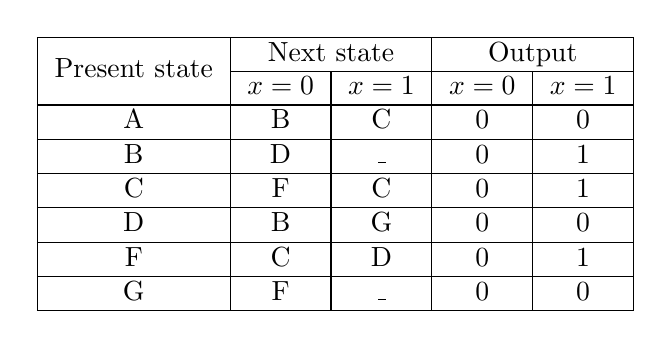
\begin{tikzpicture}
			\node(table)
			{
				\begin{tabular}{| c | c | c | c | c |}
					\hline
					\multirow{2}{*}{Present state} & \multicolumn{2}{c |}{Next state} & \multicolumn{2}{c |}{Output} \\
					\cline{2-5} & $x = 0$ & $x = 1$ & $x = 0$ & $x = 1$\\
					\hline
					A & B & C & 0 & 0 \\
					\hline
					B & D & \_ & 0 & 1 \\
					\hline
					C & F & C & 0 & 1 \\
					\hline
					D & B & G & 0 & 0 \\
					\hline
					F & C & D & 0 & 1 \\
					\hline
					G & F & \_ & 0 & 0 \\
					\hline
				\end{tabular}
			};
		\end{tikzpicture}
	\end{center}
	
	\section*{Question II}
	\subsection*{Part a}
	\begin{center}
		\begin{tikzpicture}
			\node(graphic)
			{
				\includegraphics[scale=0.8]{Q2a.pdf}
			};
		\end{tikzpicture}
	\end{center}
	
	\subsection*{Part b}
	\begin{lstlisting}[language=vhdl]
library ieee;
library altera;
use ieee.std_logic_1164.all;
use altera.altera_primitives_components.all;

entity Q2 is
    port (
        CLK: in std_logic;
        RESETN: in std_logic;
        R: in std_logic_vector(1 to 3);
        G: out std_logic_vector(1 to 3)
    );
end;


architecture Structural of Q2 is
    component DFF
        port (
            D: in std_logic;
            CLK: in std_logic;
            CLRN: in std_logic;
            PRN: in std_logic;
            Q: out std_logic
        );
    end component;
    
    signal signalD: std_logic_vector(1 downto 0);
    signal signalQ: std_logic_vector(1 downto 0);
begin
    generateDFF: for i in 1 downto 0 generate
        DFFInst: DFF
            port map (
                D => signalD(i),
                CLK => CLK,
                CLRN => RESETN,
                PRN => '1',
                Q => signalQ(i)
            );
    end generate;

    signalD(1) <=    -- (r1' + s1)r3 + ((s1 + r1)' + s1s0')r2
        ((not R(1) or signalQ(1)) and R(3))
        or (((signalQ(1) nor R(1)) or (signalQ(1) and not signalQ(0))) and R(2));
    
    signalD(0) <=    -- (r2' + s1s0)r3 + s1'r1
        ((not R(2) or (signalQ(1) and signalQ(0))) and R(3))
        or (not signalQ(1) and R(1));
    
    -- g1 = s1'r1
    G(1) <= not signalQ(1) and R(1);
    
    -- g2 = ((s1 + r1)' + s1s0')r2
    G(2) <=
        ((signalQ(1) nor R(1))
            or (signalQ(1) and not signalQ(0)))
        and R(2);
    
    -- g3 = ((r1 + r2)' + s1r2' + s1s0)r3
    G(3) <=
        ((R(1) nor R(2))
            or (signalQ(1) and not R(2))
            or (signalQ(1) and signalQ(0)))
        and R(3);
    
end;
	\end{lstlisting}
	
	\subsection*{Part c}
	Transition table:
	\begin{center}
		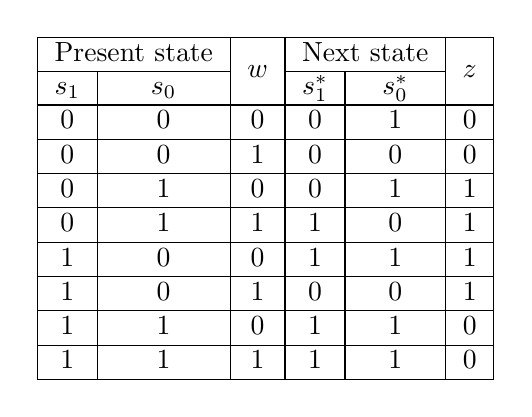
\begin{tikzpicture}
			\node(table)
			{
				\begin{tabular}{| c | c | c | c | c | c |}
					\hline
					\multicolumn{2}{| c |}{Present state} & \multirow{2}{*}{$w$} &\multicolumn{2}{c |}{Next state} & \multirow{2}{*}{$z$} \\
					\cline{1-2} \cline{4-5} $s_1$ & $s_0$ & & $s_1^*$ & $s_0^*$ & \\
					\hline
					0 & 0 & 0 & 0 & 1 & 0 \\
					\hline
					0 & 0 & 1 & 0 & 0 & 0 \\
					\hline
					0 & 1 & 0 & 0 & 1 & 1 \\
					\hline
					0 & 1 & 1 & 1 & 0 & 1 \\
					\hline
					1 & 0 & 0 & 1 & 1 & 1 \\
					\hline
					1 & 0 & 1 & 0 & 0 & 1 \\
					\hline
					1 & 1 & 0 & 1 & 1 & 0 \\
					\hline
					1 & 1 & 1 & 1 & 1 & 0 \\
					\hline
				\end{tabular}
			};
		\end{tikzpicture}
	\end{center}
	
	Transistion equations:
	\begin{align*}
		s_1^* &= s_1 + s_0w \\
		s_0^* &= w' + s_1s_0 \\
		z &= s_1 \oplus s_0
	\end{align*}
	
	Final circuit diagram:
	\begin{center}
		\begin{tikzpicture}
		\node(graphic)
		{
			\includegraphics{Q2c.pdf}
		};
		\end{tikzpicture}
	\end{center}

	\section*{Question III}
	\subsection*{Part a}
	Using sequential encoding for the transition table:
	\begin{center}
		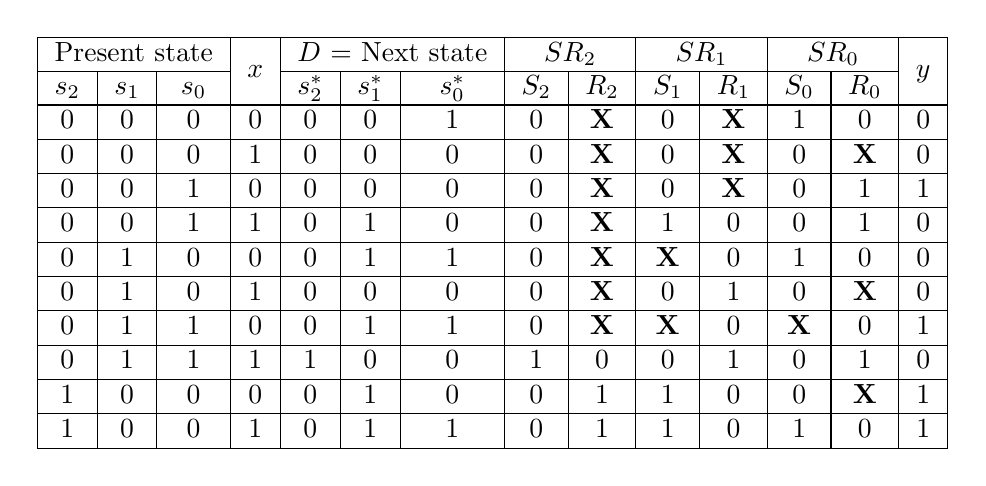
\begin{tikzpicture}
			\node(table)
			{
				\begin{tabular}{| c | c | c | c | c | c | c | c | c | c | c | c | c | c |}
					\hline
					\multicolumn{3}{| c |}{Present state} & \multirow{2}{*}{$x$} &\multicolumn{3}{c |}{$D$ = Next state} & \multicolumn{2}{c |}{$SR_2$} & \multicolumn{2}{c |}{$SR_1$} & \multicolumn{2}{c |}{$SR_0$} & \multirow{2}{*}{$y$} \\
					\cline{1-3} \cline{5-13}
					$s_2$ & $s_1$ & $s_0$ & & $s_2^*$ & $s_1^*$ & $s_0^*$ & $S_2$ & $R_2$ & $S_1$ & $R_1$ & $S_0$ & $R_0$ & \\
					\hline
					0 & 0 & 0 & 0 & 0 & 0 & 1 & 0 & \textbf{X} & 0 & \textbf{X} & 1 & 0 & 0 \\
					\hline
					0 & 0 & 0 & 1 & 0 & 0 & 0 & 0 & \textbf{X} & 0 & \textbf{X} & 0 & \textbf{X} & 0 \\
					\hline
					0 & 0 & 1 & 0 & 0 & 0 & 0 & 0 & \textbf{X} & 0 & \textbf{X} & 0 & 1 & 1 \\
					\hline
					0 & 0 & 1 & 1 & 0 & 1 & 0 & 0 & \textbf{X} & 1 & 0 & 0 & 1 & 0 \\
					\hline
					0 & 1 & 0 & 0 & 0 & 1 & 1 & 0 & \textbf{X} & \textbf{X} & 0 & 1 & 0 & 0 \\
					\hline
					0 & 1 & 0 & 1 & 0 & 0 & 0 & 0 & \textbf{X} & 0 & 1 & 0 & \textbf{X} & 0 \\
					\hline
					0 & 1 & 1 & 0 & 0 & 1 & 1 & 0 & \textbf{X} & \textbf{X} & 0 & \textbf{X} & 0 & 1 \\
					\hline
					0 & 1 & 1 & 1 & 1 & 0 & 0 & 1 & 0 & 0 & 1 & 0 & 1 & 0 \\
					\hline
					1 & 0 & 0 & 0 & 0 & 1 & 0 & 0 & 1 & 1 & 0 & 0 & \textbf{X} & 1 \\
					\hline
					1 & 0 & 0 & 1 & 0 & 1 & 1 & 0 & 1 & 1 & 0 & 1 & 0 & 1 \\
					\hline
				\end{tabular}
			};
		\end{tikzpicture}
	\end{center}
	
	Transition equations for D flip-flop:
	\begin{equation}
		\begin{aligned}
			s_2^* &= s_1s_0x \\
			s_1^* &= s_2 + s_1x' + s_1's_0x \\
			s_0^* &= s_1x' + s_2x + s_2's_0'x'
		\end{aligned}
	\end{equation}
	
	Transition equations for SR flip-flop:
	\begin{equation}
		\begin{aligned}
			S_2 &= s_1s_0x \\
			R_2 &= s_1' \\
			S_1 &= s_2 + s_1's_0x \\
			R_1 &= s_1x \\
			S_0 &= s_2x + s_2's_0'x' \\
			R_0 &= s_2'x + s_1's_0
		\end{aligned}
	\end{equation}
	
	Transition equations for the output:
	\begin{equation}
		\begin{aligned}
			y &= s_2 + s_0x'
		\end{aligned}
	\end{equation}

	
	Final circuit diagram:
	\begin{center}
		\begin{tikzpicture}
		\node(graphic)[label=below:Circuit Using D Flip-flops]
		{
			\includegraphics[scale=0.9]{Q3aD.pdf}
		};
		\end{tikzpicture}
	\end{center}
	
	\begin{center}
		\begin{tikzpicture}
		\node(graphic)[label=below:Circuit Using SR Flip-flops]
		{
			\includegraphics{Q3aSR.pdf}
		};
		\end{tikzpicture}
	\end{center}
	
	\subsection*{Part b}
	Grouping possible adjacent states:
	
	By Rule 1, $(CD)$ and $(AC)$ can be two adjacency groups;
	
	By Rule 2, $(BA)$, $(AC)$, $(DA)$, $(DE)$ and $(CD)$ can be five adjacency groups;
	
	By Rule 3, $(AC)$, $(BCE)$ and $(ABCD)$ can be three adjacency groups;
	\\
	\\
	Satisfy the adjancy relations above by Rule priority:
	\begin{center}
		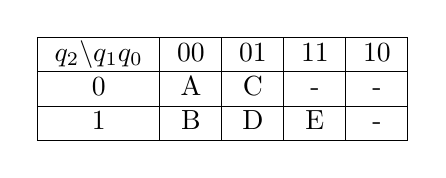
\begin{tikzpicture}
			\node(table)
			{
				\begin{tabular}{| c | c | c | c | c |}
					\hline
					$q_2$\textbackslash$q_1q_0$ & 00 & 01 & 11 & 10 \\
					\hline
					0 & A & C & - & - \\
					\hline
					1 & B & D & E & - \\
					\hline
				\end{tabular}
			};
		\end{tikzpicture}
	\end{center}
	
	State assignment:
	\begin{align*}
		A &= 000 \\
		B &= 100 \\
		C &= 001 \\
		D &= 101 \\
		E &= 111
	\end{align*}
	
	Transition table:
	\begin{center}
		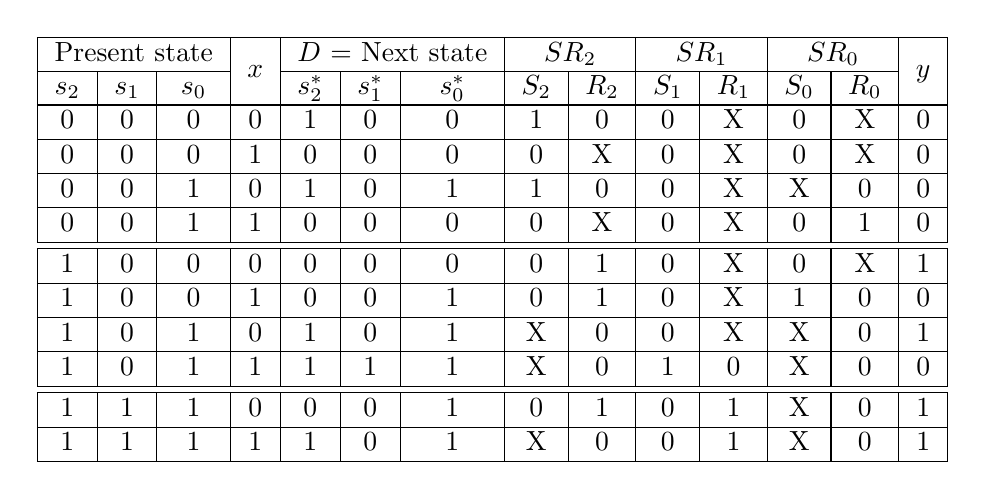
\begin{tikzpicture}
			\node(table)
			{
				\begin{tabular}{| c | c | c | c | c | c | c | c | c | c | c | c | c | c |}
					\hline
					\multicolumn{3}{| c |}{Present state} & \multirow{2}{*}{$x$} &\multicolumn{3}{c |}{$D$ = Next state} & \multicolumn{2}{c |}{$SR_2$} & \multicolumn{2}{c |}{$SR_1$} & \multicolumn{2}{c |}{$SR_0$} & \multirow{2}{*}{$y$} \\
					\cline{1-3} \cline{5-13}
					$s_2$ & $s_1$ & $s_0$ & & $s_2^*$ & $s_1^*$ & $s_0^*$ & $S_2$ & $R_2$ & $S_1$ & $R_1$ & $S_0$ & $R_0$ & \\
					\hline
					0 & 0 & 0 & 0 & 1 & 0 & 0 & 1 & 0 & 0 & X & 0 & X & 0 \\
					\hline
					0 & 0 & 0 & 1 & 0 & 0 & 0 & 0 & X & 0 & X & 0 & X & 0 \\
					\hline
					0 & 0 & 1 & 0 & 1 & 0 & 1 & 1 & 0 & 0 & X & X & 0 & 0 \\
					\hline
					0 & 0 & 1 & 1 & 0 & 0 & 0 & 0 & X & 0 & X & 0 & 1 & 0 \\
					\hline
					\hline
					1 & 0 & 0 & 0 & 0 & 0 & 0 & 0 & 1 & 0 & X & 0 & X & 1 \\
					\hline
					1 & 0 & 0 & 1 & 0 & 0 & 1 & 0 & 1 & 0 & X & 1 & 0 & 0 \\
					\hline
					1 & 0 & 1 & 0 & 1 & 0 & 1 & X & 0 & 0 & X & X & 0 & 1 \\
					\hline
					1 & 0 & 1 & 1 & 1 & 1 & 1 & X & 0 & 1 & 0 & X & 0 & 0 \\
					\hline
					\hline
					1 & 1 & 1 & 0 & 0 & 0 & 1 & 0 & 1 & 0 & 1 & X & 0 & 1 \\
					\hline
					1 & 1 & 1 & 1 & 1 & 0 & 1 & X & 0 & 0 & 1 & X & 0 & 1 \\
					\hline
				\end{tabular}
			};
		\end{tikzpicture}
	\end{center}
	
	Transition equations for D flip-flop:
	\begin{equation}
		\begin{aligned}
			s_2^* &= s_2'x' + s_1x + s_2s_1's_0 \\
			s_1^* &= s_2s_1's_0x \\
			s_0^* &= s_0x' + s_2x
		\end{aligned}
	\end{equation}
	
	Transition equations for SR flip-flop:
	\begin{equation}
		\begin{aligned}
			S_2 &= s_2'x' \\
			R_2 &= s_1x' + s_2s_0' \\
			S_1 &= s_2s_1's_0x \\
			R_1 &= s_1 \\
			S_0 &= s_2x \\
			R_0 &= s_2'x
		\end{aligned}
	\end{equation}
	
	Transition equations for the output:
	\begin{equation}
		\begin{aligned}
			y &= s_1 + s_2x'
		\end{aligned}
	\end{equation}
	
	The complexity of the transition equations has decresed, especially for the circuit that uses SR flip-flops.
\end{document}
